\documentclass[12pt,a4paper]{article}

\usepackage{float}
\usepackage[utf8]{inputenc}
\usepackage[T1]{fontenc}
\usepackage[ngerman]{babel}
\usepackage{geometry}
\usepackage{hyperref}
\usepackage{booktabs}
\usepackage{enumitem}
\usepackage{fancyhdr}
\usepackage{titlesec}
\usepackage{graphicx}
\usepackage{textcomp}
\geometry{left=2.5cm,right=2.5cm,top=2.5cm,bottom=2.5cm}

\pagestyle{fancy}
\fancyhf{}
\lhead{ePortfolio -- Künstliche Intelligenz}
\rhead{Bahaa Alnahar}
\cfoot{\thepage}

\titleformat{\section}{\Large\bfseries}{\thesection}{1em}{}[\titlerule]

\begin{document}

\begin{titlepage}
\centering
\vspace*{2cm}

{\Huge \textbf{ePortfolio}}\\[0.5cm]
{\Large Vorlesung: Methoden der KI}\\[1.5cm]

\begin{tabular}{ll}
Name: & Bahaa Alnahar \\
Matrikelnummer: & 2117485 \\
Studiengang: & International Information Systems \\
Hochschule: & Technische Hochschule Augsburg \\
Pruefungsformat: & Portfolio-Pruefung \\
Abgabe: & 19.07.2026 \\
\end{tabular}

\vfill
{\large Sommersemester 2026}

\end{titlepage}

\tableofcontents
\newpage

\section{Einleitung}

Dieses ePortfolio dokumentiert meine Bearbeitung der Aufgaben aus der Vorlesung
\textit{Methoden der KI}. Ziel ist es, die Inhalte nicht nur zusammenzufassen,
sondern auch eigene Experimente, Beobachtungen und Reflexionen zu dokumentieren.

\newpage

\section{Blatt 1: Einfuehrung in KI}

\subsection{Aufgabe 1: KI-Tools testen und bewerten}

\subsubsection*{Ziel}

In dieser Aufgabe habe ich verschiedene KI-Tools aus den vorgegebenen Webseiten getestet.
Ziel war es zu analysieren, was gut funktioniert und wo Schwachstellen liegen.

\subsubsection*{Tool 1: theresanaiforthat.com}

Ich habe die Webseite \textit{theresanaiforthat.com} besucht und den Bereich
\textit{Trending} analysiert.

\begin{figure}[h]
    \centering
    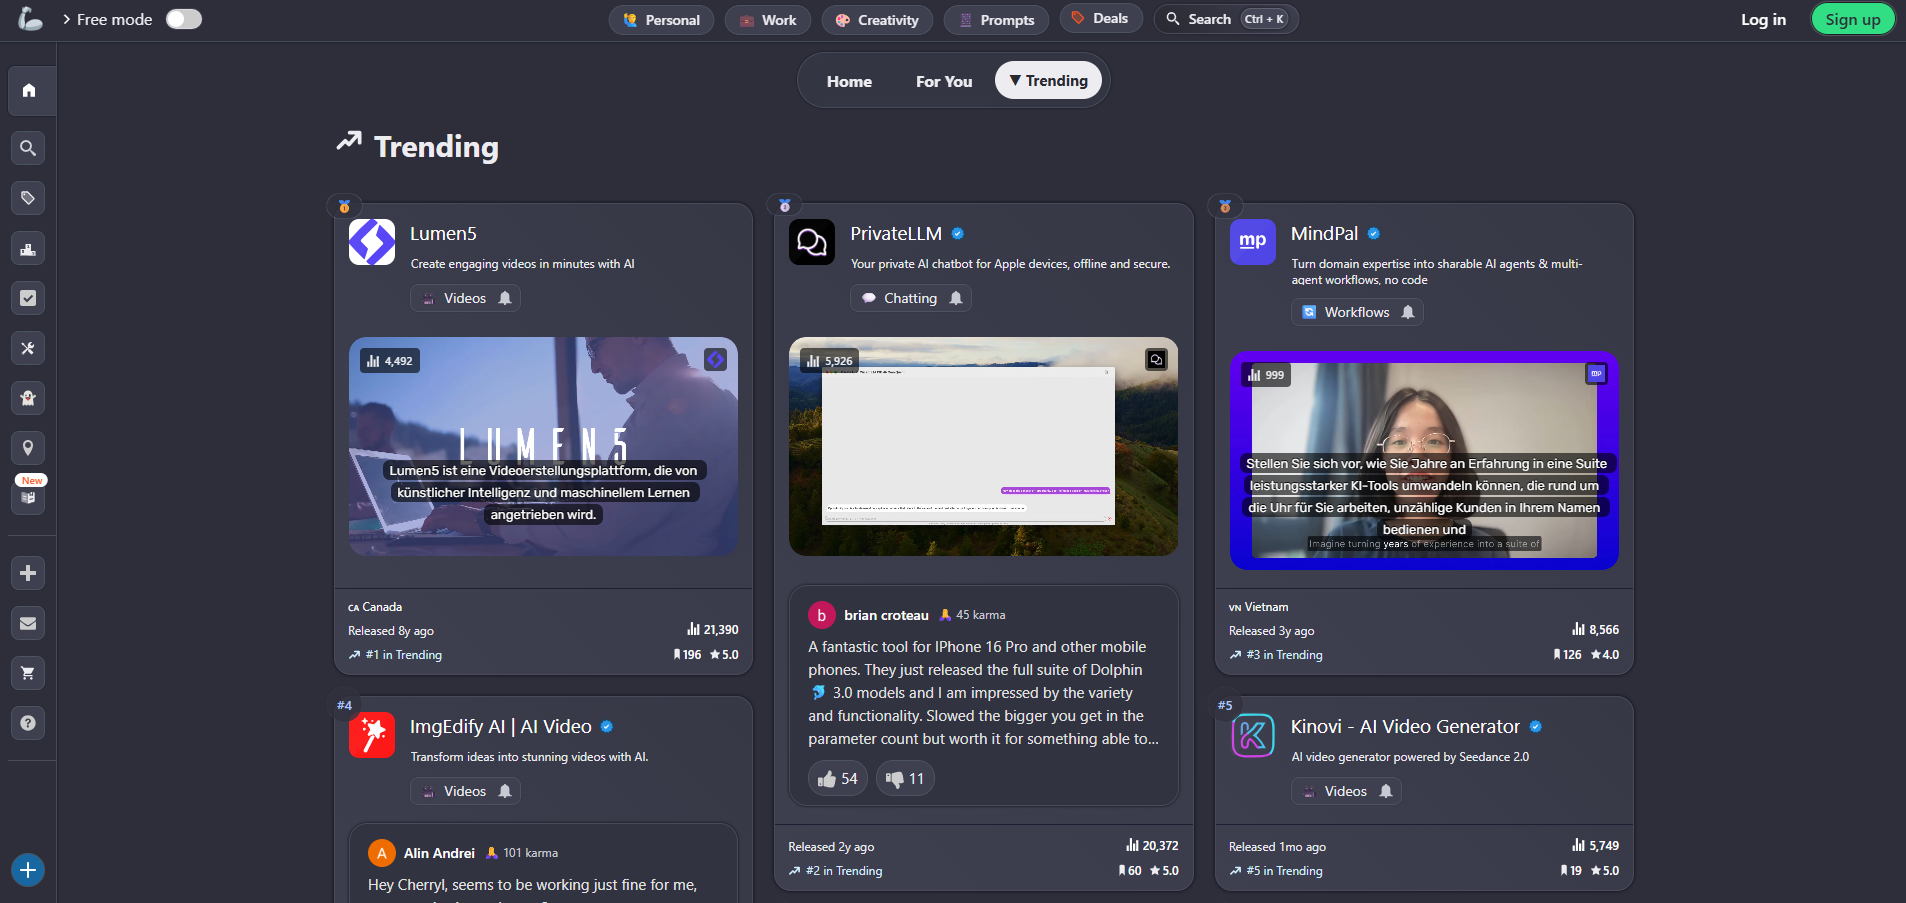
\includegraphics[width=0.9\textwidth]{figures/ai_tools_trending.png}
    \caption{Trending KI-Tools auf theresanaiforthat.com}
\end{figure}

\textbf{Beobachtung:}

Die Webseite zeigt viele aktuelle KI-Tools wie:
\begin{itemize}
    \item Lumen5 (Video-Erstellung mit KI)
    \item PrivateLLM (lokaler Chatbot)
    \item MindPal (KI-Agenten und Workflows)
\end{itemize}

\textbf{Was funktioniert gut:}
\begin{itemize}
    \item Sehr viele aktuelle Tools
    \item Gute Uebersicht (Trending, Kategorien)
    \item Man sieht direkt, wofuer die Tools genutzt werden
\end{itemize}

\textbf{Schwachstellen:}
\begin{itemize}
    \item Viele Tools brauchen Login oder Bezahlung
    \item Keine tiefe Bewertung der Qualitaet
    \item Man muss selbst entscheiden, welches Tool gut ist
\end{itemize}

\textbf{Reflexion:}

Die Seite zeigt deutlich, wie schnell sich KI entwickelt.
Es gibt sehr viele Anwendungen, besonders im Bereich Video, Chatbots und Automatisierung.
Allerdings ist es schwierig zu erkennen, welche Tools wirklich gut sind.
\subsubsection*{Tool 2: ml5.js Beispiele}

ml5.js bietet interaktive Machine-Learning-Demos direkt im Browser.

\textbf{Was funktioniert gut:}
\begin{itemize}
    \item Sehr anschaulich und visuell
    \item Einfach zu bedienen (kein Setup notwendig)
    \item Gut zum Lernen von ML-Grundlagen
\end{itemize}

\textbf{Schwachstellen:}
\begin{itemize}
    \item Nur einfache Beispiele
    \item Nicht fuer reale Projekte geeignet
    \item Begrenzte Daten und Modelle
\end{itemize}

\textbf{Reflexion:}

ml5.js ist perfekt fuer Einsteiger. Es hilft, Machine Learning besser zu verstehen,
aber fuer echte Anwendungen braucht man leistungsfaehigere Tools.

\subsubsection*{Tool 3: Azure AI Services}

Azure bietet professionelle KI-Services, z.B. fuer Sprache, Bilderkennung und Textanalyse.

\textbf{Was funktioniert gut:}
\begin{itemize}
    \item Sehr leistungsfaehige Modelle
    \item Viele verschiedene Funktionen (Vision, Speech, NLP)
    \item Einsatz in realen Unternehmen moeglich
\end{itemize}

\textbf{Schwachstellen:}
\begin{itemize}
    \item Komplex in der Nutzung
    \item Registrierung notwendig
    \item Kosten fuer Nutzung
\end{itemize}

\textbf{Reflexion:}

Azure zeigt, wie KI in der Praxis eingesetzt wird. Im Vergleich zu einfachen Tools ist es viel
maechtiger, aber auch schwieriger zu bedienen.

\subsubsection*{Zwischenfazit}

Die getesteten Tools zeigen, dass KI heute in vielen Bereichen eingesetzt wird.
Es gibt einfache Lern-Tools wie ml5.js und professionelle Systeme wie Azure.
Trotz der Fortschritte gibt es weiterhin Probleme wie Kosten, Komplexitaet und
unterschiedliche Qualitaet der Ergebnisse.

\subsection{Teil b: Entwicklung der KI in den letzten 15 Jahren}

\subsubsection*{Ziel}

In diesem Teil der Aufgabe soll untersucht werden, wie sich Künstliche Intelligenz
in den letzten 15 Jahren entwickelt hat.

\subsubsection*{KI-Anwendungen im Jahr 2010}

Im Jahr 2010 waren KI-Anwendungen deutlich eingeschränkter als heute.
Typische Beispiele sind:

\begin{itemize}
    \item Siri (erste Version als Sprachassistent)
    \item Google Voice Search (Spracherkennung)
    \item Netflix Empfehlungssystem
    \item Pandora Music Empfehlungssystem
    \item LinkedIn "People You May Know"
\end{itemize}

Diese Systeme waren sogenannte \textbf{Narrow AI}, also auf eine einzelne Aufgabe spezialisiert.

\subsubsection*{Eigenschaften von KI im Jahr 2010}

\begin{itemize}
    \item KI war auf einzelne Aufgaben begrenzt
    \item Systeme konnten nicht flexibel denken
    \item Kein echtes Verstaendnis von Sprache
    \item Kaum generative Faehigkeiten (kein Text oder Bild erzeugen)
\end{itemize}

\subsubsection*{KI-Anwendungen heute (2025/2026)}

Heute hat sich KI stark weiterentwickelt. Beispiele sind:

\begin{itemize}
    \item ChatGPT, Gemini, Claude (LLM-Chatbots)
    \item Bildgeneratoren wie DALL-E oder Midjourney
    \item Coding-Assistenten
    \item KI-Agenten und Automatisierungssysteme
\end{itemize}

\subsubsection*{Unterschiede zwischen 2010 und heute}

\begin{itemize}
    \item Frueher: Spezialisierte Systeme (Narrow AI)
    \item Heute: Allgemeinere Systeme (General AI-Ansatz)
    \item Frueher: Fokus auf Erkennung (Speech, Recommendation)
    \item Heute: Generative KI (Text, Bilder, Code)
    \item Frueher: KI im Hintergrund
    \item Heute: KI als direkter Assistent fuer Nutzer
\end{itemize}

\subsubsection*{Was faellt auf?}

Die Entwicklung der KI ist sehr schnell verlaufen.
Besonders auffaellig ist der Wechsel von spezialisierten Systemen
zu vielseitigen, generativen Modellen.

Heute kann KI nicht nur analysieren, sondern auch Inhalte erzeugen.
Das fuehrt zu neuen Moeglichkeiten, aber auch zu Risiken wie
Fehlinformationen oder Abhaengigkeit von KI-Systemen.

\subsubsection*{Reflexion}

Ich finde besonders interessant, wie schnell sich KI entwickelt hat.
Vor 15 Jahren war KI kaum sichtbar fuer normale Nutzer.
Heute ist sie ein fester Bestandteil im Alltag und im Studium.

Trotzdem ist es wichtig, KI kritisch zu betrachten und ihre Grenzen zu verstehen.
\subsection{Aufgabe 2: Grenzen heutiger KI-Systeme}

\subsubsection*{Aufgabenverstaendnis}

In dieser Aufgabe sollen zwei Beispiele genannt werden, die Menschen gut
bewaeltigen koennen, KI-Systeme oder Roboter jedoch noch nicht zuverlaessig loesen.

\subsubsection*{Beispiel 1: Flexibles Handeln in einer unstrukturierten Umgebung}

Ein Mensch kann sich in einer neuen Wohnung schnell orientieren, Hindernisse erkennen
und spontan darauf reagieren (z.B. Gegenstaende verschieben oder umgehen).

\textbf{Begruendung:}

Menschen kombinieren visuelle Wahrnehmung, Erfahrung und Intuition.
KI-Roboter hingegen benoetigen genaue Modelle der Umgebung und haben Schwierigkeiten
mit unerwarteten Situationen.

\subsubsection*{Beispiel 2: Verstehen von sozialen Situationen und Emotionen}

Menschen koennen oft erkennen, ob jemand traurig, ironisch oder unsicher ist.
Sie verstehen auch indirekte Aussagen oder Humor.

\textbf{Begruendung:}

Soziale Kommunikation basiert stark auf Kontext, Kultur und Erfahrung.
KI-Systeme koennen zwar Sprache analysieren, aber echtes Verstaendnis und Empathie
sind weiterhin schwierig.

\subsubsection*{Fazit}

Diese Beispiele zeigen, dass KI in klar definierten Aufgaben sehr stark ist.
In offenen, komplexen und sozialen Situationen sind Menschen jedoch noch ueberlegen.

\subsubsection*{Vergleich verschiedener Uebersetzungsdienste}

Ich habe den folgenden deutschen Satz mit zwei verschiedenen
Uebersetzungsdiensten getestet:

\textbf{Original:}

Wieder ist ein Jahr vergangen: allmaehlich wird mir dieser ewig waehrende Zyklus ein wenig leid.

\textbf{DeepL:}

Another year has gone by: I'm starting to get a little tired of this never-ending cycle.

\textbf{Google Translate:}

Another year has passed: I'm gradually getting a little tired of this never-ending cycle.

\subsubsection*{Analyse}

Beide Uebersetzungen sind korrekt, unterscheiden sich jedoch leicht:

\begin{itemize}
    \item DeepL verwendet \textit{"I'm starting to get tired"}, was natuerlicher klingt
    \item Google verwendet \textit{"I'm gradually getting tired"}, was naeher am Wort \textit{"allmaehlich"} ist
    \item Beide Systeme verstehen die allgemeine Bedeutung des Satzes
\end{itemize}

\subsubsection*{Was faellt auf?}

Auch wenn beide Systeme gute Ergebnisse liefern, gibt es Unterschiede im Stil und in der Genauigkeit.
Dies zeigt, dass maschinelle Uebersetzung keine perfekte Loesung ist.

\subsubsection*{Reflexion}

Maschinelle Uebersetzungsdienste funktionieren heute sehr gut bei komplexen Saetzen.
Trotzdem gibt es Unterschiede in der Wortwahl und im Stil.
Deshalb sollte man wichtige Uebersetzungen immer kritisch pruefen.
\subsection{Aufgabe 4: Autonomes Fahren / Selbstlenkende Autos}



\subsubsection*{Aktueller Stand}

Autonomes Fahren ist heute nicht mehr nur Forschung, sondern wird in einigen Regionen
bereits praktisch eingesetzt. Besonders weit ist Waymo in den USA. Waymo bietet
autonome Fahrdienste unter anderem in Phoenix, San Francisco und Los Angeles an.
In Phoenix kann man bereits ein autonomes Fahrzeug ueber die Waymo-App bestellen.
\cite{waymo_phoenix}

Auch Deutschland ist relevant: Mercedes-Benz bietet mit DRIVE PILOT ein System fuer
bedingt automatisiertes Fahren nach SAE Level 3 an. Dabei darf das Fahrzeug unter
bestimmten Bedingungen Fahraufgaben uebernehmen, der Fahrer muss aber weiterhin
uebernahmebereit bleiben. \cite{mercedes_drive_pilot}

\subsubsection*{Laender und Beispiele}

\begin{itemize}
    \item \textbf{USA:} Robotaxi-Dienste, besonders durch Waymo.
    \item \textbf{Deutschland:} Level-3-Systeme wie Mercedes-Benz DRIVE PILOT.
    \item \textbf{China:} Robotaxi-Projekte, zum Beispiel Baidu Apollo Go. Gleichzeitig zeigen aktuelle Berichte, dass Behoerden wegen Sicherheits- und Kontrollfragen strenger werden. \cite{china_av}
    \item \textbf{Singapur:} Tests und Vorbereitung autonomer Shuttle-Dienste, aber weiterhin Herausforderungen bei Haftung und Regulierung. \cite{singapore_av}
\end{itemize}

\subsubsection*{Schwierigkeiten}

Trotz grosser Fortschritte gibt es noch viele Probleme:

\begin{itemize}
    \item \textbf{Komplexe Verkehrssituationen:} Baustellen, Fussgaenger, Radfahrer und unerwartete Hindernisse sind schwierig.
    \item \textbf{Wetter:} Starker Regen, Schnee oder Nebel koennen Sensoren stoeren.
    \item \textbf{Haftung:} Es ist nicht immer klar, wer bei einem Unfall verantwortlich ist: Fahrer, Hersteller oder Softwareanbieter.
    \item \textbf{Regulierung:} Gesetze muessen festlegen, wo und unter welchen Bedingungen autonome Fahrzeuge fahren duerfen.
    \item \textbf{Vertrauen:} Viele Menschen vertrauen autonomen Fahrzeugen noch nicht vollstaendig.
    \item \textbf{Datenschutz und Cybersecurity:} Autonome Fahrzeuge sammeln viele Daten und muessen gegen Angriffe geschuetzt werden.
\end{itemize}

\subsubsection*{Reflexion}

Autonomes Fahren zeigt gut, dass KI in der realen Welt viel schwieriger ist als in einer
kontrollierten Demo. Ein Fahrzeug muss nicht nur Verkehrsregeln kennen, sondern auch
unsichere und neue Situationen richtig einschaetzen. Besonders interessant finde ich,
dass es schon echte Anwendungen gibt, aber der Einsatz stark von Land, Gesetzgebung
und Sicherheitsanforderungen abhaengt.

\subsubsection*{Fazit}

Autonomes Fahren ist bereits in bestimmten Bereichen im Einsatz, vor allem bei Robotaxis
in den USA und Level-3-Systemen in Deutschland. Vollstaendig autonomes Fahren ueberall
und unter allen Bedingungen ist aber noch nicht erreicht.
\subsection{Aufgabe 5: Superhuman AI und Singularity}
Ich denke, dass KI in Zukunft in vielen Bereichen besser als Menschen werden kann.
Heute sieht man das schon bei Datenanalyse oder beim Schreiben von Text.

Trotzdem glaube ich nicht,
dass Maschinen Menschen komplett ersetzen koennen.
Menschen haben Emotionen, Erfahrungen und soziale Faehigkeiten,
die fuer KI schwer nachzubilden sind.

Positiv finde ich,
dass KI Menschen im Alltag oder im Studium helfen kann.
Auch gefaehrliche Arbeiten koennten von Maschinen uebernommen werden.

Andererseits sehe ich auch Risiken.
Zum Beispiel koennten manche Arbeitsplaetze verschwinden
oder Menschen koennten sich zu stark auf KI verlassen.

Wichtig finde ich deshalb,
dass es klare Regeln fuer KI gibt
und dass Menschen weiterhin wichtige Entscheidungen kontrollieren.

\subsubsection*{ChatGPT-Antwort}

\textbf{a) Wie realistisch sind Superhuman AI oder Singularity?}

Superhuman AI beschreibt KI-Systeme, die Menschen in vielen intellektuellen
Bereichen uebertreffen koennten. Der Begriff Singularity bezeichnet einen
moeglichen Zeitpunkt, an dem KI-Systeme sich selbst verbessern und dadurch
sehr schnell leistungsfaehiger werden.

Aus heutiger Sicht ist es realistisch, dass KI Menschen in spezialisierten
Aufgaben uebertrifft. Bereits heute sind KI-Systeme in Bereichen wie
Schach, Bilderkennung, Datenanalyse oder Sprachverarbeitung oft besser
oder schneller als Menschen.

Ob jedoch eine allgemeine Superintelligenz entsteht, die Menschen in
allen Bereichen uebertrifft, ist weiterhin umstritten.
Viele Wissenschaftler halten dies fuer moeglich, andere sehen darin
eher Spekulation.

\bigskip

\textbf{b) Welche positiven und negativen Folgen koennte Superhuman AI haben?}

Moegliche positive Folgen waeren:

\begin{itemize}
    \item Fortschritte in Medizin und Wissenschaft
    \item Schnellere Analyse grosser Datenmengen
    \item Automatisierung gefaehrlicher Arbeiten
    \item Unterstuetzung bei Bildung und Forschung
    \item Effizientere Prozesse in Unternehmen und Industrie
\end{itemize}

Moegliche negative Folgen waeren:

\begin{itemize}
    \item Verlust von Arbeitsplaetzen
    \item Missbrauch fuer Manipulation oder Ueberwachung
    \item Abhaengigkeit von KI-Systemen
    \item Konzentration von Macht bei wenigen Unternehmen
    \item Sicherheitsrisiken durch autonome Systeme
\end{itemize}

\bigskip

\textbf{c) Welche Massnahmen sollten ergriffen werden?}

Um Risiken zu reduzieren, sollten verschiedene Massnahmen umgesetzt werden:

\begin{itemize}
    \item Entwicklung klarer gesetzlicher Regelungen fuer KI
    \item Transparenz und Nachvollziehbarkeit von KI-Entscheidungen
    \item Schutz personenbezogener Daten
    \item Internationale Zusammenarbeit bei KI-Regeln
    \item Forschung zu KI-Sicherheit und KI-Ethik
    \item Bildung ueber Chancen und Risiken von KI
\end{itemize}

Viele Ethik-Diskussionen fordern ausserdem,
dass Menschen weiterhin Kontrolle ueber wichtige Entscheidungen behalten sollten.

\subsection{Aufgabe 6: Denken und Think-Aloud-Methode}

\subsubsection*{a) Versuch, nicht zu denken}

Der Versuch ist mir nicht gelungen.
Schon nach kurzer Zeit sind automatisch Gedanken aufgetaucht.

\subsubsection*{b) Woran habe ich gedacht?}

Ich habe an die Aufgabe selbst gedacht und mich gefragt,
wie man ueberhaupt fuer einige Sekunden nicht denken kann.

\subsubsection*{c) Wie nehme ich mein Denken wahr?}

Ich nehme mein Denken oft als eine Art inneres Gespraech mit mir selbst wahr.
Dabei ueberlege ich verschiedene Szenarien
und versuche vorherzusagen, was passieren koennte oder welche Entscheidung sinnvoll waere.

\subsubsection*{d) Think-Aloud-Methode}

Ich habe die Think-Aloud-Methode beim Besuch eines Online-Shops ausprobiert.
Dabei habe ich laut ausgesprochen, was ich gerade suche oder denke.

Zum Beispiel habe ich mich gefragt:

\begin{itemize}
    \item Was kann ich hier Nuetzliches kaufen?
    \item Welche Angebote gibt es?
    \item Ist ein Produkt wirklich guenstig?
    
\end{itemize}

Dabei ist mir aufgefallen,
dass man beim Benutzen einer Webseite staendig Erwartungen,
Fragen und Bewertungen im Kopf hat.

\subsubsection*{Reflexion}

Die Aufgabe hat gezeigt,
dass Denken oft automatisch passiert.
Ausserdem wurde deutlich,
dass Menschen beim Verwenden von Webseiten viele innere Entscheidungen treffen,
die fuer das Design von Benutzeroberflaechen wichtig sind.


\newpage
\section{Vertiefung: Von Daten zu lernenden und erklaerbaren KI-Systemen}

\subsection*{Warum diese Reihenfolge?}

Für mein ePortfolio ordne ich die Themen bewusst nicht zufällig, sondern entlang eines fachlichen roten Fadens. Ziel ist es, einen vollständigen KI-Prozess sichtbar zu machen: von der Analyse der Daten über das Lernen von Modellen bis hin zur kritischen Bewertung und Erklärbarkeit der Ergebnisse.

\begin{enumerate}
\item \textbf{Data Mining:} Am Anfang steht die systematische Untersuchung von Daten. Dabei werden Muster, Strukturen, Zusammenhänge und Auffälligkeiten erkannt. Data Mining bildet damit die Grundlage, um aus Rohdaten verwertbare Informationen zu gewinnen.

```
\item \textbf{Machine Learning:} Aufbauend auf den erkannten Datenstrukturen werden Modelle trainiert, die aus Beispielen lernen und Vorhersagen oder Klassifikationen treffen können. Machine Learning zeigt, wie aus Daten lernfähige Systeme entstehen.

\item \textbf{Deep Learning:} Anschließend werden komplexere Modellarchitekturen betrachtet, insbesondere neuronale Netze. Deep Learning ist besonders relevant für große Datenmengen und komplexe Anwendungsfelder wie Bildverarbeitung, Sprachverarbeitung und moderne Large Language Models.

\item \textbf{Erklärbare KI / XAI:} Abschließend wird untersucht, wie KI-Entscheidungen nachvollziehbar, interpretierbar und kritisch bewertbar gemacht werden können. Dies ist wichtig, weil leistungsfähige Modelle nicht nur gute Ergebnisse liefern sollen, sondern auch transparent, vertrauenswürdig und verantwortungsvoll eingesetzt werden müssen.
```

\end{enumerate}

Diese Reihenfolge ist wichtig, weil moderne KI nicht nur aus einem einzelnen Algorithmus besteht. Ein vollständiges KI-System benötigt Daten, Vorverarbeitung, Modellbildung, Training, Evaluation und Erklärbarkeit. Dadurch kann ich im Portfolio nicht nur theoretische Grundlagen darstellen, sondern auch einen praktischen und reflektierten KI-Prozess .

\begin{table}[h]
\centering
\begin{tabular}{p{3cm}p{4cm}p{4cm}p{3cm}}
\toprule
\textbf{Thema} & \textbf{Ziel} & \textbf{Typisches Experiment} & \textbf{Reflexionsfrage} \\
\midrule
Data Mining & Muster in Daten entdecken & Datenanalyse und Visualisierung & Was sagen die Daten ueber das Problem? \\
Machine Learning & Aus Daten Vorhersagen lernen & Klassifikation mit Entscheidungsbaum oder kNN & Generalisiert das Modell auf neue Daten? \\
Deep Learning & Komplexe Muster mit neuronalen Netzen lernen & MLP oder Bildklassifikation & Ist ein komplexes Modell wirklich notwendig? \\
Erklaerbare KI & Entscheidungen nachvollziehbar machen & Entscheidungsbaum visualisieren oder SHAP/LIME testen & Kann ein Mensch die Entscheidung verstehen? \\
\bottomrule
\end{tabular}
\caption{Vergleich von Data Mining, Machine Learning, Deep Learning und erklaerbarer KI}
\end{table}.
\subsection{Mein methodisches Vorgehen im Portfolio}

Fuer jedes Thema verwende ich dieselbe wissenschaftliche Struktur:

\begin{enumerate}
    \item \textbf{Begriffsklaerung}: Was bedeutet der Begriff?
    \item \textbf{Bedeutung}: Warum ist das Thema fuer KI relevant?
    \item \textbf{Praktisches Experiment}: Welche kleine Implementierung oder Demo habe ich getestet?
    \item \textbf{Beobachtung}: Was ist im Experiment passiert?
    \item \textbf{Reflexion}: Was habe ich daraus gelernt und wo liegen Grenzen?
\end{enumerate}




\subsection{Data Mining: Muster in Daten entdecken}

\subsubsection*{Begriffsklärung}

Data Mining bezeichnet den Prozess, aus größeren Datenbeständen nicht-triviale, bislang unbekannte und potenziell nützliche Muster und Zusammenhänge zu extrahieren.\cite{witten_data_mining,fayyad_kdd} Im Unterschied zur reinen Datenverarbeitung liegt der Fokus nicht nur auf dem Speichern, Sortieren oder Abfragen von Daten, sondern auf dem Gewinnen neuen Wissens aus vorhandenen Daten.\cite{witten_data_mining} Data Mining kann dabei statistische Verfahren, Visualisierungen und Methoden des Machine Learning kombinieren, um Strukturen in Daten sichtbar zu machen.\cite{han_data_mining}

\subsubsection*{Warum ist Data Mining wichtig?}

Data Mining ist wichtig, weil große Datenbestände häufig Muster enthalten, die mit einer rein manuellen oder klassischen Analyse leicht übersehen werden.\cite{ibm_data_mining,haufe_data_mining} Durch die systematische Analyse solcher Daten können Organisationen datengetriebene Entscheidungen treffen, zum Beispiel im Marketing, in der Produktion, im Finanzbereich oder in der Prozessoptimierung.\cite{inform_data_mining}

In Unternehmen ermöglicht Data Mining unter anderem, Kundensegmente zu identifizieren, Churn-Risiken früh zu erkennen, Betrug aufzudecken und Prozesse effizienter zu gestalten.\cite{haufe_data_mining,ibm_data_mining} Damit bildet Data Mining eine wichtige Grundlage für moderne KI-Systeme, weil vor dem Training eines Machine-Learning-Modells zunächst verstanden werden muss, welche Daten vorliegen, welche Merkmale relevant sind und ob erkennbare Muster existieren.

\subsubsection*{Einordnung des verwendeten Datensatzes}

Für das praktische Experiment wurde der Iris-Datensatz verwendet. Dieser Datensatz geht auf Ronald A. Fisher zurück und gehört zu den klassischen Beispieldatensätzen in Statistik, Data Mining und Machine Learning.\cite{fisher_iris} Er enthält Messwerte verschiedener Iris-Blumenarten und wird häufig genutzt, um grundlegende Methoden der Datenanalyse und Klassifikation verständlich zu demonstrieren.\cite{sklearn_iris}

Im Datensatz werden drei Iris-Arten betrachtet: \textit{Iris setosa}, \textit{Iris versicolor} und \textit{Iris virginica}. Jede Beobachtung beschreibt eine einzelne Blume anhand von vier numerischen Merkmalen: Länge und Breite der Kelchblätter sowie Länge und Breite der Blütenblätter. Die englischen Begriffe \textit{sepal} und \textit{petal} bedeuten dabei:

\begin{itemize}
\item \textbf{sepal:} Kelchblatt der Blume
\item \textbf{petal:} Blütenblatt der Blume
\item \textbf{petal length:} Länge des Blütenblatts in Zentimetern
\item \textbf{petal width:} Breite des Blütenblatts in Zentimetern
\end{itemize}

Diese Einordnung ist wichtig, weil die Visualisierung nicht nur abstrakte Zahlenwerte zeigt, sondern reale biologische Merkmale, anhand derer sich verschiedene Iris-Arten unterscheiden lassen. Dadurch eignet sich der Datensatz gut, um den Übergang von Data Mining zu Machine Learning nachvollziehbar zu erklären.

\subsubsection*{Experimentidee für das ePortfolio}

Ziel des Experiments ist es, den Iris-Datensatz explorativ zu untersuchen und erste Muster in den Daten sichtbar zu machen. Dabei soll noch kein Machine-Learning-Modell trainiert werden. Stattdessen steht das grundlegende Verstehen der Daten im Vordergrund.

\textbf{Vorgehen:}

\begin{enumerate}
\item Datensatz laden.
\item Spalten, Datentypen und fehlende Werte untersuchen.
\item Ausgewählte Merkmale visualisieren.
\item Erste Muster beschreiben und interpretieren.
\end{enumerate}

\subsubsection*{Umsetzung des Experiments}

Für das Data-Mining-Experiment wurde ein eigenes Python-Skript erstellt und lokal ausgeführt. Ziel war es, den Iris-Datensatz nicht sofort mit einem Machine-Learning-Modell zu klassifizieren, sondern ihn zunächst explorativ zu untersuchen. Dadurch sollten erste Muster, Unterschiede und mögliche Zusammenhänge in den Daten sichtbar gemacht werden.

\begin{itemize}
\item \textbf{Datei:} \texttt{DM.py}
\item \textbf{Ordner:} \texttt{code/01_data_mining}
\item \textbf{Datensatz:} Iris-Datensatz aus \texttt{scikit-learn}
\item \textbf{Bibliotheken:} \texttt{pandas}, \texttt{matplotlib}, \texttt{scikit-learn}
\end{itemize}

Der Code wurde schrittweise nachvollzogen, an die eigene Projektstruktur angepasst und in der lokalen Entwicklungsumgebung ausgeführt. Zur Unterstützung bei der Strukturierung des Skripts sowie bei der Fehlerbehebung wurde ChatGPT verwendet. Die fachliche Interpretation der Ergebnisse, die Auswahl der Visualisierung und die Reflexion der Erkenntnisse erfolgten eigenständig im Rahmen dieses ePortfolios.

Das Skript lädt zunächst den Iris-Datensatz und wandelt ihn in eine tabellarische Datenstruktur um. Anschließend werden die ersten Datensätze, die vorhandenen Merkmale, die Datentypen, statistische Kennzahlen sowie mögliche fehlende Werte untersucht. Diese Schritte sind wichtig, weil Data Mining nicht mit einem Modell beginnt, sondern mit dem systematischen Verstehen der Daten.

Im nächsten Schritt werden die numerischen Zielklassen in verständliche Klassennamen umgewandelt. Dadurch können die drei Iris-Arten \textit{setosa}, \textit{versicolor} und \textit{virginica} in der Visualisierung direkt interpretiert werden.

\subsubsection*{Visualisierung und Interpretation}

Zur Visualisierung möglicher Muster wurden die Merkmale \textit{petal length} und \textit{petal width} in einem Streudiagramm gegenübergestellt. Diese beiden Merkmale wurden ausgewählt, weil sie besonders gut zeigen, wie sich die drei Iris-Arten voneinander unterscheiden. Abbildung~\ref{fig:iris-scatterplot} zeigt, dass bereits eine einfache zweidimensionale Darstellung deutliche Strukturen im Datensatz sichtbar machen kann.

\begin{figure}[htbp]
\centering
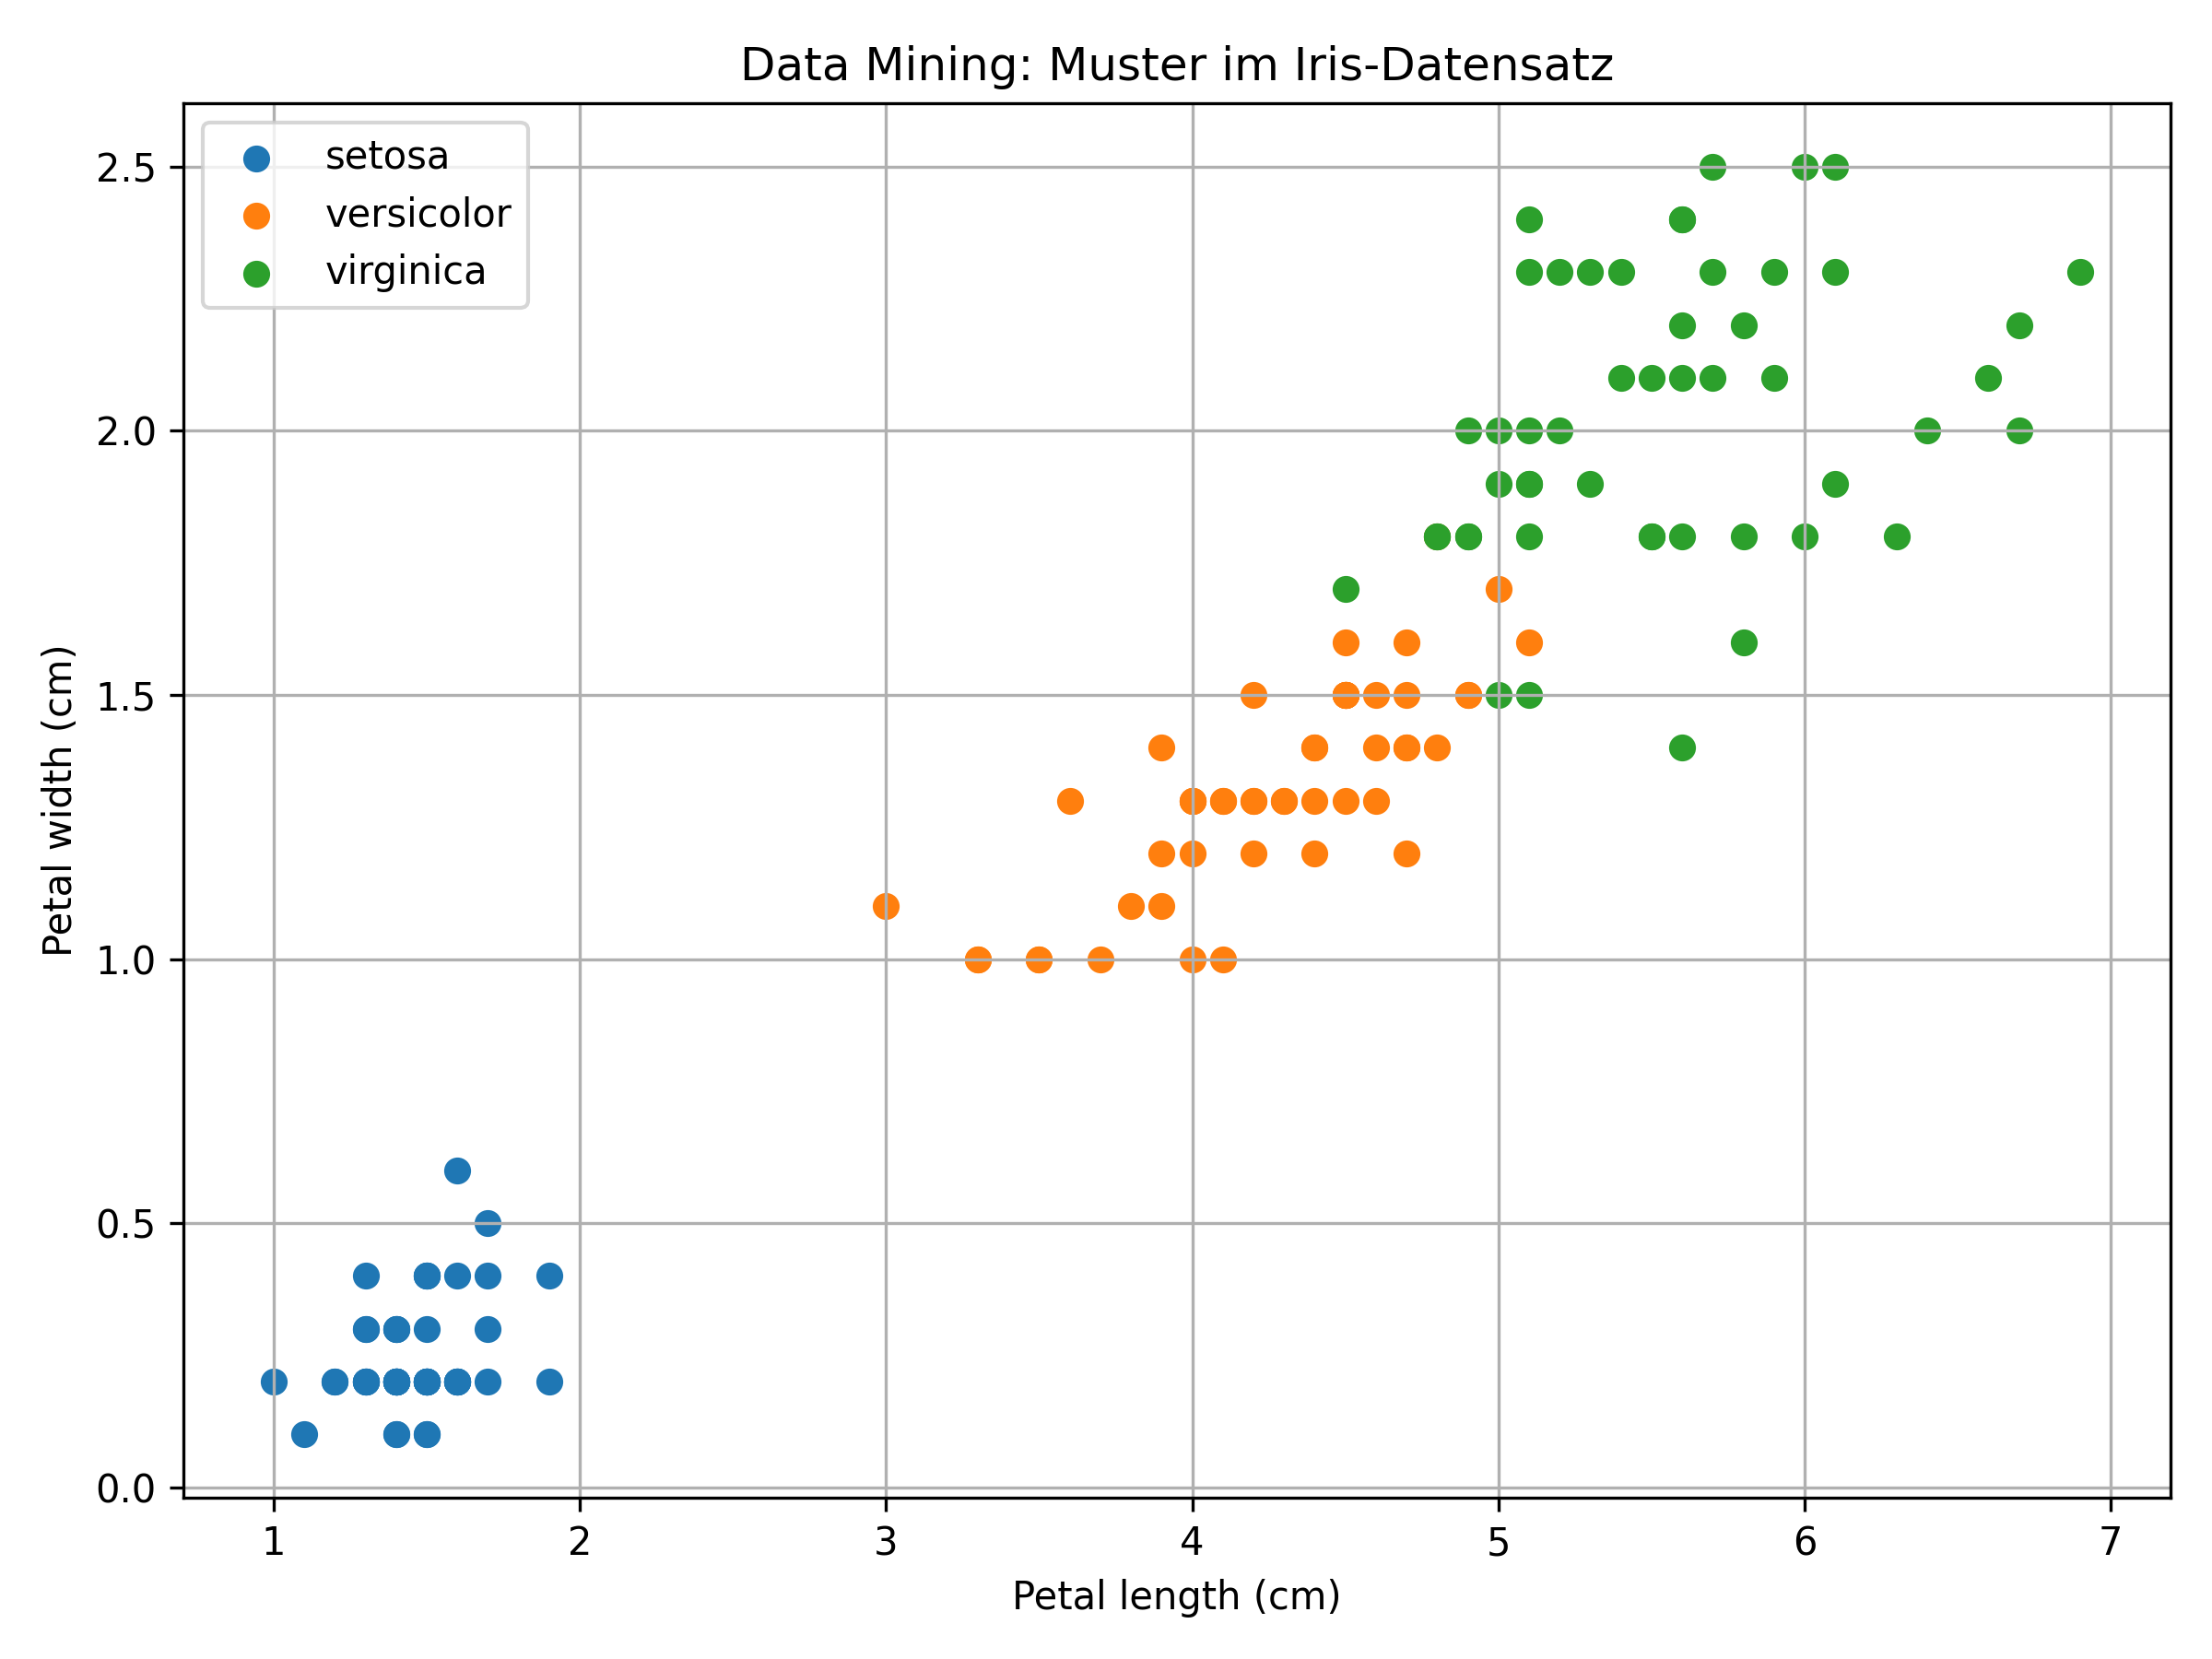
\includegraphics[width=0.85\textwidth]{figures/iris_scatterplot.png}
\caption{Streudiagramm der Merkmale \textit{petal length} und \textit{petal width} im Iris-Datensatz. Die Visualisierung zeigt, dass sich die Iris-Art \textit{setosa} deutlich von den anderen beiden Arten abgrenzt.}
\label{fig:iris-scatterplot}
\end{figure}

In der Visualisierung ist erkennbar, dass sich die Klasse \textit{setosa} deutlich von den anderen beiden Klassen unterscheidet. Die Klassen \textit{versicolor} und \textit{virginica} liegen näher beieinander und weisen teilweise Überschneidungen auf. Daraus lässt sich ableiten, dass die Merkmale \textit{petal length} und \textit{petal width} für eine spätere Klassifikation relevant sein können.

Gleichzeitig zeigt die Darstellung eine Grenze einfacher Visualisierungen: Es werden nur zwei Merkmale betrachtet. Der Iris-Datensatz enthält jedoch insgesamt vier numerische Merkmale. Für ein vollständigeres Verständnis wären daher weitere Visualisierungen oder eine anschließende Machine-Learning-Analyse sinnvoll.

\subsubsection*{Reflexion}

Durch dieses Experiment wurde deutlich, dass Data Mining ein wichtiger Schritt vor dem eigentlichen Machine Learning ist. Bevor ein Modell trainiert wird, muss zunächst verstanden werden, welche Daten vorliegen, welche Merkmale relevant sein könnten und ob erkennbare Muster existieren.

Besonders auffällig war, dass sich \textit{Iris setosa} bereits mit zwei Merkmalen klar von den anderen Arten unterscheiden lässt. Dies zeigt, dass einfache explorative Methoden bereits wertvolle Hinweise für spätere Modellierungsentscheidungen liefern können. Gleichzeitig wurde sichtbar, dass eine einzelne Visualisierung nicht ausreicht, um die gesamte Datenstruktur vollständig zu erfassen.

Für mein ePortfolio ist dieses Experiment deshalb wichtig, weil es den Übergang von theoretischem Wissen zu praktischer Datenanalyse zeigt. Ich dokumentiere nicht nur, was Data Mining bedeutet, sondern auch, wie erste Muster mit Python sichtbar gemacht und kritisch interpretiert werden können.
\subsection{Aufgabe 3: k-Means-Clustering und k-Nächste-Nachbarn}

In Aufgabe 3 wird untersucht, ob sich anhand verschiedener Wachstumsfaktoren natürliche Gruppen innerhalb einer kleinen Pflanzendatenmenge bilden lassen. Die gegebene Tabelle enthält insgesamt 16 Datenpunkte mit den Merkmalen Feuchte, Säuregrad, durchschnittliche Temperaturminima und Wachstum. Für die Teilaufgabe 3a sollen zunächst nur die ersten zehn Datenpunkte verwendet und mit dem k-Means-Verfahren in zwei Cluster eingeteilt werden. Dabei ist vorgegeben, dass $k=2$ gilt und die Datenpunkte 1 und 8 als initiale Clusterzentren verwendet werden. Anschließend sollen in Teilaufgabe 3b die Datenpunkte 11 und 16 mithilfe des k-Nächste-Nachbarn-Verfahrens den zuvor entstandenen Clustern zugeordnet werden .

\subsubsection{Ziel der Aufgabe}

Das Ziel dieser Aufgabe besteht darin, den Unterschied und den Zusammenhang zwischen Clustering und Klassifikation praktisch zu verstehen. Beim Clustering werden Datenpunkte ohne vorgegebene Zielklasse in Gruppen eingeteilt. Das Verfahren versucht also, Ähnlichkeiten in den Eingabedaten selbst zu erkennen. Im Gegensatz dazu ordnet ein Klassifikationsverfahren neue Datenpunkte bereits bekannten Klassen oder Gruppen zu.

In dieser Aufgabe wird zuerst mit k-Means ein Clustering durchgeführt. Danach werden neue Datenpunkte mithilfe von k-Nächste-Nachbarn einem bereits bestehenden Cluster zugeordnet. Dadurch wird sichtbar, wie ein unüberwachtes Lernverfahren und ein einfaches Zuordnungsverfahren kombiniert werden können.

\subsubsection{Datenvorbereitung}

Das k-Means-Verfahren kann nicht direkt mit textuellen Kategorien wie \textit{trocken}, \textit{feucht}, \textit{basisch} oder \textit{neutral} rechnen. Deshalb mussten die kategorialen Merkmale zunächst in numerische Werte umgewandelt werden. Für diese Aufgabe wurde folgende Kodierung verwendet:

\begin{itemize}
    \item Feuchte:
    \begin{itemize}
        \item trocken = 0
        \item feucht = 1
    \end{itemize}
    \item Säure:
    \begin{itemize}
        \item basisch = 0
        \item neutral = 1
        \item alkalisch = 2
    \end{itemize}
\end{itemize}

Das Merkmal Temperatur wurde unverändert übernommen, da es bereits numerisch vorliegt. Das Merkmal Wachstum wurde für das Clustering nicht verwendet, weil k-Means ein unüberwachtes Verfahren ist. Das bedeutet, dass die Gruppen allein anhand der Eingabemerkmale Feuchte, Säuregrad und Temperatur gebildet werden.

\subsubsection{Kodierte Datenpunkte}

Die ersten zehn Datenpunkte werden nach der Kodierung wie folgt dargestellt:

\begin{table}[h]
\centering
\begin{tabular}{c|c|c|c|c}
\hline
Nr. & Feuchte & Säure & Temp. & Kodierter Vektor \\
\hline
1 & trocken & basisch & 7 & $(0,0,7)$ \\
2 & feucht & neutral & 8 & $(1,1,8)$ \\
3 & trocken & neutral & 7 & $(0,1,7)$ \\
4 & feucht & alkalisch & 5 & $(1,2,5)$ \\
5 & trocken & neutral & 8 & $(0,1,8)$ \\
6 & trocken & neutral & 6 & $(0,1,6)$ \\
7 & trocken & neutral & 11 & $(0,1,11)$ \\
8 & trocken & neutral & 9 & $(0,1,9)$ \\
9 & trocken & alkalisch & 9 & $(0,2,9)$ \\
10 & trocken & alkalisch & 8 & $(0,2,8)$ \\
\hline
\end{tabular}
\caption{Kodierte Darstellung der ersten zehn Datenpunkte}
\end{table}

\subsubsection{Durchführung des k-Means-Verfahrens}

Für die Clusteranalyse wurde $k=2$ gewählt. Das bedeutet, dass die Datenpunkte in zwei Cluster aufgeteilt werden sollen. Die Aufgabe gibt außerdem vor, dass die Datenpunkte 1 und 8 als initiale Clusterzentren verwendet werden. Daraus ergeben sich zu Beginn folgende Zentren:

\[
C_1^{(0)} = DP_1 = (0,0,7)
\]

\[
C_2^{(0)} = DP_8 = (0,1,9)
\]

Die Zuordnung der Datenpunkte erfolgt anhand der euklidischen Distanz. Für zwei Punkte

\[
x = (x_1,x_2,x_3)
\]

und

\[
y = (y_1,y_2,y_3)
\]

ergibt sich die Distanz durch:

\[
d(x,y) = \sqrt{(x_1-y_1)^2 + (x_2-y_2)^2 + (x_3-y_3)^2}
\]

Jeder Datenpunkt wird demjenigen Clusterzentrum zugeordnet, zu dem seine Distanz am kleinsten ist.

\subsubsection{Erste Zuordnung der Datenpunkte}

Nach der Berechnung der Distanzen zu den beiden initialen Clusterzentren ergibt sich folgende Zuordnung:

\[
Cluster\ 1 = \{1,3,4,6\}
\]

\[
Cluster\ 2 = \{2,5,7,8,9,10\}
\]

Die erste Gruppe enthält also die Datenpunkte 1, 3, 4 und 6. Die zweite Gruppe enthält die Datenpunkte 2, 5, 7, 8, 9 und 10.

\subsubsection{Berechnung der neuen Clusterzentren}

Im nächsten Schritt werden die Clusterzentren neu berechnet. Dazu wird für jedes Cluster der Mittelwert der enthaltenen Datenpunkte gebildet.

Für Cluster 1 gilt:

\[
DP_1 = (0,0,7)
\]

\[
DP_3 = (0,1,7)
\]

\[
DP_4 = (1,2,5)
\]

\[
DP_6 = (0,1,6)
\]

Das neue Zentrum von Cluster 1 ergibt sich aus dem Mittelwert dieser vier Punkte:

\[
C_1 = 
\left(
\frac{0+0+1+0}{4},
\frac{0+1+2+1}{4},
\frac{7+7+5+6}{4}
\right)
\]

\[
C_1 = (0.25, 1.00, 6.25)
\]

Für Cluster 2 gilt:

\[
DP_2 = (1,1,8)
\]

\[
DP_5 = (0,1,8)
\]

\[
DP_7 = (0,1,11)
\]

\[
DP_8 = (0,1,9)
\]

\[
DP_9 = (0,2,9)
\]

\[
DP_{10} = (0,2,8)
\]

Das neue Zentrum von Cluster 2 ergibt sich aus dem Mittelwert dieser sechs Punkte:

\[
C_2 =
\left(
\frac{1+0+0+0+0+0}{6},
\frac{1+1+1+1+2+2}{6},
\frac{8+8+11+9+9+8}{6}
\right)
\]

\[
C_2 = (0.17, 1.33, 8.83)
\]

\subsubsection{Konvergenz des Verfahrens}

Nach der Neuberechnung der Clusterzentren wird die Zuordnung der Datenpunkte erneut überprüft. Dabei bleibt die Zuordnung unverändert:

\[
Cluster\ 1 = \{1,3,4,6\}
\]

\[
Cluster\ 2 = \{2,5,7,8,9,10\}
\]

Da sich die Clusterzuordnung nicht mehr ändert, ist das k-Means-Verfahren konvergiert. Die finalen Clusterzentren lauten:

\[
C_1 = (0.25, 1.00, 6.25)
\]

\[
C_2 = (0.17, 1.33, 8.83)
\]

\subsubsection{Interpretation der k-Means-Ergebnisse}

Die Ergebnisse zeigen, dass Cluster 1 hauptsächlich Datenpunkte mit niedrigeren Temperaturwerten enthält. Die Temperaturwerte in Cluster 1 liegen bei 5, 6 und 7 Grad. Cluster 2 enthält dagegen überwiegend Datenpunkte mit höheren Temperaturwerten zwischen 8 und 11 Grad.

Damit scheint die Temperatur in dieser konkreten Kodierung einen besonders starken Einfluss auf die Clusterbildung zu haben. Das liegt daran, dass die Temperaturwerte numerisch einen größeren Wertebereich besitzen als die kodierten Kategorien für Feuchte und Säuregrad. Ohne Normalisierung können solche Merkmale das Ergebnis des k-Means-Verfahrens dominieren.

\subsubsection{Zuordnung der Datenpunkte 11 und 16 mit k-Nächste-Nachbarn}

In Teilaufgabe 3b sollen die Datenpunkte 11 und 16 den zuvor gebildeten Clustern zugeordnet werden. Dazu werden die beiden Datenpunkte zunächst ebenfalls numerisch kodiert.

Datenpunkt 11 lautet in der Tabelle:

\[
DP_{11} = \text{feucht, basisch, 7}
\]

Mit der oben definierten Kodierung ergibt sich:

\[
DP_{11} = (1,0,7)
\]

Datenpunkt 16 lautet:

\[
DP_{16} = \text{trocken, basisch, 4}
\]

Damit ergibt sich:

\[
DP_{16} = (0,0,4)
\]

Für die Zuordnung werden die Distanzen der neuen Datenpunkte zu den finalen Clusterzentren berechnet.

Für Datenpunkt 11 gilt:

\[
d(DP_{11}, C_1)
=
\sqrt{(1-0.25)^2 + (0-1.00)^2 + (7-6.25)^2}
\]

\[
d(DP_{11}, C_1)
=
\sqrt{0.75^2 + (-1.00)^2 + 0.75^2}
\]

\[
d(DP_{11}, C_1)
=
\sqrt{0.5625 + 1 + 0.5625}
=
\sqrt{2.125}
\approx 1.46
\]

Die Distanz zu Clusterzentrum 2 beträgt:

\[
d(DP_{11}, C_2)
=
\sqrt{(1-0.17)^2 + (0-1.33)^2 + (7-8.83)^2}
\]

\[
d(DP_{11}, C_2)
\approx 2.42
\]

Da

\[
1.46 < 2.42
\]

gilt, wird Datenpunkt 11 dem ersten Cluster zugeordnet:

\[
DP_{11} \rightarrow Cluster\ 1
\]

Für Datenpunkt 16 gilt:

\[
d(DP_{16}, C_1)
=
\sqrt{(0-0.25)^2 + (0-1.00)^2 + (4-6.25)^2}
\]

\[
d(DP_{16}, C_1)
=
\sqrt{(-0.25)^2 + (-1.00)^2 + (-2.25)^2}
\]

\[
d(DP_{16}, C_1)
=
\sqrt{0.0625 + 1 + 5.0625}
=
\sqrt{6.125}
\approx 2.47
\]

Die Distanz zu Clusterzentrum 2 beträgt:

\[
d(DP_{16}, C_2)
=
\sqrt{(0-0.17)^2 + (0-1.33)^2 + (4-8.83)^2}
\]

\[
d(DP_{16}, C_2)
\approx 5.02
\]

Da

\[
2.47 < 5.02
\]

gilt, wird auch Datenpunkt 16 dem ersten Cluster zugeordnet:

\[
DP_{16} \rightarrow Cluster\ 1
\]

\subsubsection{Endergebnis}

Die finale Clusterstruktur für die ersten zehn Datenpunkte lautet:

\[
Cluster\ 1 = \{1,3,4,6\}
\]

\[
Cluster\ 2 = \{2,5,7,8,9,10\}
\]

Die neuen Datenpunkte werden wie folgt zugeordnet:

\[
DP_{11} \rightarrow Cluster\ 1
\]

\[
DP_{16} \rightarrow Cluster\ 1
\]

\subsubsection{Kritische Reflexion}

Die Aufgabe zeigt, dass die Anwendung von k-Means stark von der Datenvorbereitung abhängt. Da mehrere Merkmale kategorial vorliegen, mussten sie zunächst numerisch kodiert werden. Diese Kodierung ist jedoch nicht vollständig neutral. Wenn beispielsweise basisch = 0, neutral = 1 und alkalisch = 2 gesetzt wird, entsteht eine künstliche Ordnung zwischen den Kategorien. Diese Ordnung muss fachlich nicht zwingend sinnvoll sein.

Ein weiterer wichtiger Punkt ist die Skalierung der Merkmale. Die Temperatur besitzt in dieser Aufgabe einen größeren Wertebereich als die kodierten Kategorien für Feuchte und Säuregrad. Dadurch beeinflusst sie die euklidische Distanz stärker als die anderen Merkmale. Dies erklärt, warum die resultierenden Cluster vor allem nach niedrigeren und höheren Temperaturwerten getrennt werden.

Für eine professionellere Analyse wäre es sinnvoll, die Daten vor dem Clustering zu normalisieren. Alternativ könnten Verfahren verwendet werden, die besser für kategoriale Merkmale geeignet sind, zum Beispiel k-Modes oder hierarchisches Clustering mit einem passenden Distanzmaß. Dadurch könnte überprüft werden, ob die Clusterstruktur stabil bleibt oder ob sie hauptsächlich durch die gewählte Kodierung entstanden ist.

Interessant ist außerdem, dass das Zielmerkmal Wachstum nicht direkt in die Clusterbildung einbezogen wurde. Dadurch kann nachträglich analysiert werden, ob die gefundenen Cluster mit gutem oder schlechtem Wachstum zusammenhängen. In den gegebenen Daten ist dieser Zusammenhang nicht vollständig eindeutig. Das verdeutlicht eine wichtige Grenze des unüberwachten Lernens: Ein mathematisch gebildeter Cluster muss anschließend fachlich interpretiert werden.

\subsubsection{Eigene Lernreflexion}

Durch diese Aufgabe wurde deutlich, dass k-Means nicht nur aus einer einfachen Rechenvorschrift besteht, sondern mehrere methodische Entscheidungen voraussetzt. Besonders wichtig sind die Auswahl der Merkmale, die Kodierung kategorialer Daten, die Wahl der initialen Clusterzentren und die verwendete Distanzfunktion. Kleine Änderungen in diesen Entscheidungen können zu anderen Ergebnissen führen.

Für mein ePortfolio ist diese Aufgabe deshalb besonders relevant, weil sie zeigt, wie ein theoretisches Verfahren praktisch auf eine kleine Datenmenge angewendet werden kann. Gleichzeitig werden typische Grenzen des Verfahrens sichtbar. Ich habe gelernt, dass ein gutes Ergebnis im Data Mining nicht nur aus der Anwendung eines Algorithmus entsteht, sondern aus einer reflektierten Kombination von Datenverständnis, Vorverarbeitung, Berechnung und kritischer Interpretation.
\subsection{Machine Learning: Lernen aus Beispielen}

\subsubsection*{Begriffsklärung}

Machine Learning bezeichnet Verfahren, bei denen ein System aus Beispieldaten lernt, um anschließend Vorhersagen oder Klassifikationen für neue, zuvor nicht gesehene Datenpunkte zu treffen. Im Unterschied zum Data Mining steht hier nicht nur das Entdecken von Mustern im Vordergrund, sondern das Trainieren eines Modells, das diese Muster auf neue Fälle anwenden kann.

Im Rahmen dieses ePortfolios wird Machine Learning als nächster Schritt nach der explorativen Datenanalyse betrachtet. Während im Data-Mining-Teil erste Strukturen im Iris-Datensatz sichtbar wurden, soll nun überprüft werden, ob ein Klassifikator diese Strukturen nutzen kann, um die Iris-Art automatisch vorherzusagen.

\subsubsection*{Ziel des Experiments}

Ziel dieses Experiments ist es, mithilfe eines Decision-Tree-Modells die Iris-Art anhand der numerischen Merkmale \texttt{SepalLengthCm}, \texttt{SepalWidthCm}, \texttt{PetalLengthCm} und \texttt{PetalWidthCm} vorherzusagen. Die Zielvariable ist die Spalte \texttt{Species}, die die drei Klassen \texttt{Iris-setosa}, \texttt{Iris-versicolor} und \texttt{Iris-virginica} enthält.

Für die Umsetzung wurde KNIME verwendet, da der visuelle Workflow die einzelnen Schritte eines Machine-Learning-Prozesses nachvollziehbar macht: Datenimport, Aufteilung der Daten, Training des Modells, Vorhersage, Aggregation der Ergebnisse und Bewertung der Modellleistung.

\subsubsection*{Umsetzung des KNIME-Workflows}

Der Iris-Datensatz wurde zunächst mit dem \texttt{CSV Reader} in KNIME importiert. Anschließend wurde der \texttt{X-Partitioner} verwendet, um eine 10-fache Kreuzvalidierung durchzuführen. Als Klassenvariable wurde \texttt{Species} ausgewählt. Durch die Einstellung \textit{Stratified sampling} wird sichergestellt, dass die drei Iris-Arten in den jeweiligen Trainings- und Testteilen möglichst gleichmäßig vertreten sind.

Das Modell wurde mit dem \texttt{Decision Tree Learner} trainiert. Danach wurden die Testdaten jedes Validierungsdurchlaufs mit dem \texttt{Decision Tree Predictor} klassifiziert. Die Vorhersagen aller Durchläufe wurden anschließend mit dem \texttt{X-Aggregator} zusammengeführt und mit dem \texttt{Scorer} ausgewertet.


\begin{figure}[H]
    \centering
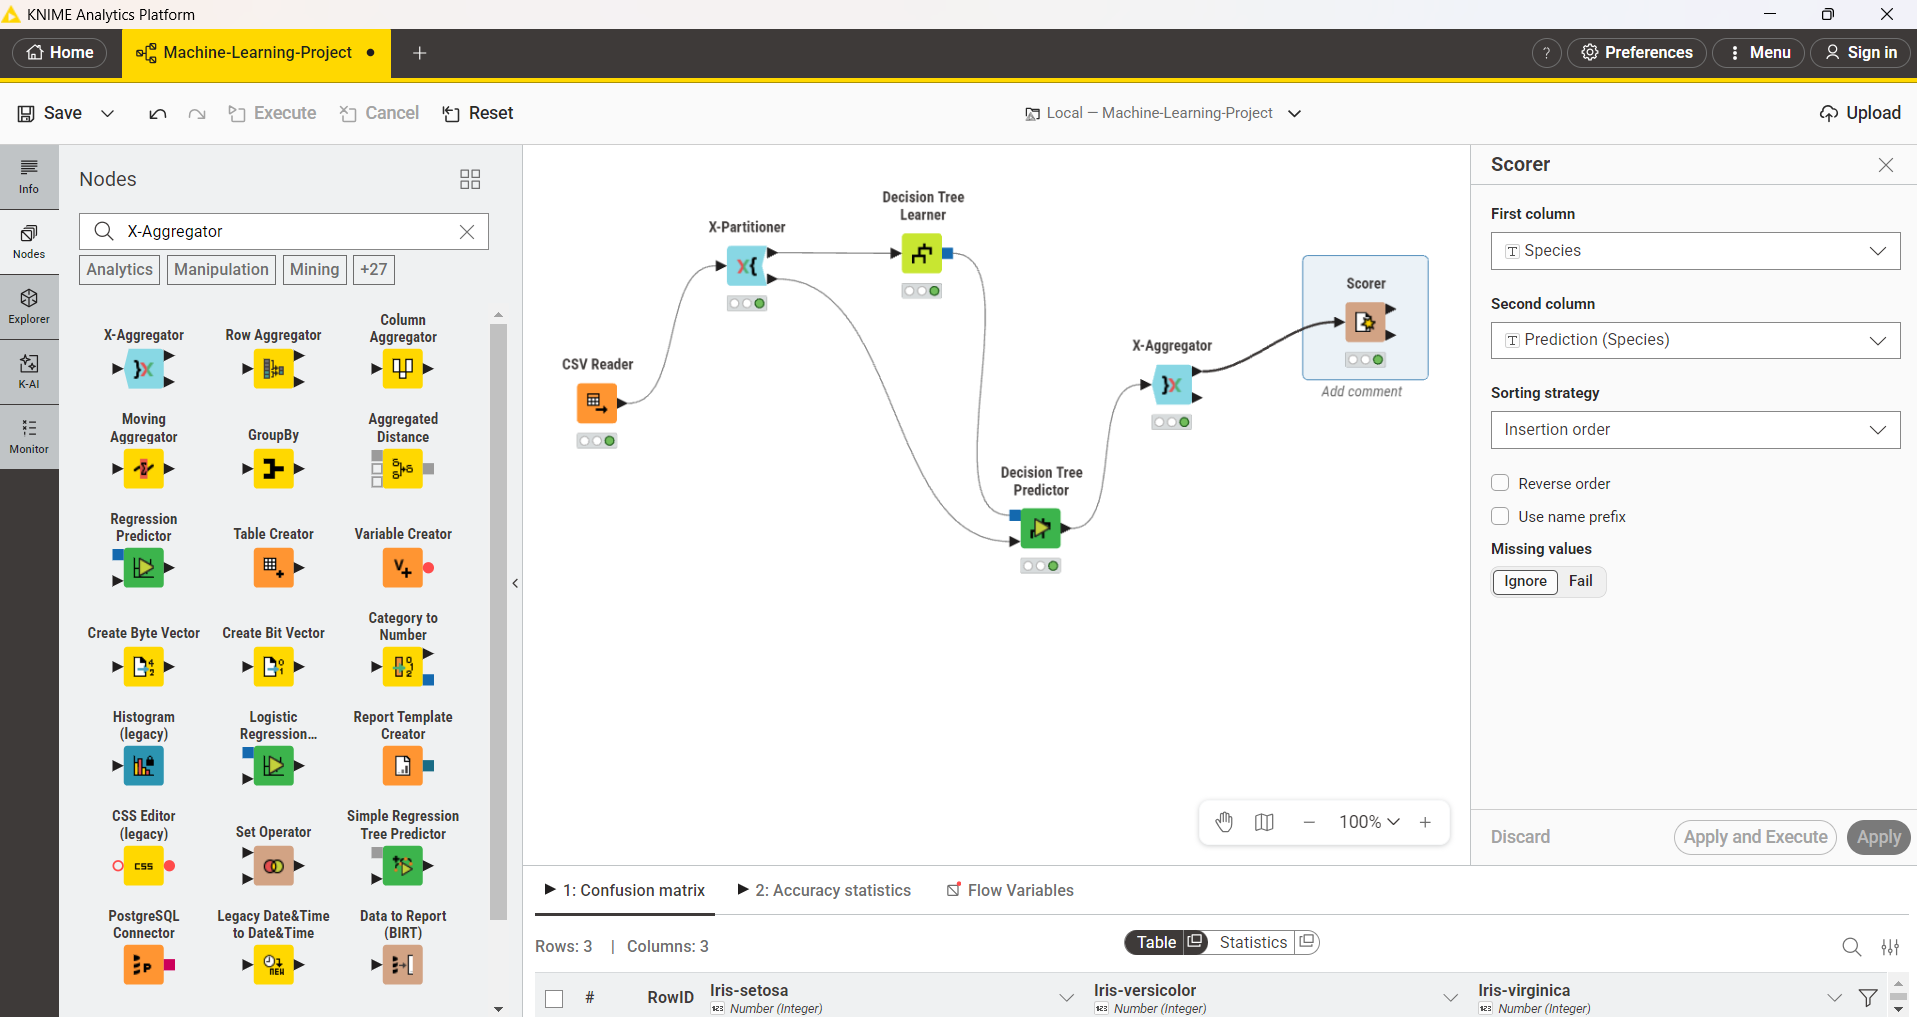
\includegraphics[width=0.95\textwidth]{figures/ml_knime_decision_tree_workflow.png}
    \caption{KNIME-Workflow zur Klassifikation des Iris-Datensatzes mit einem Decision Tree und 10-facher Kreuzvalidierung.}
    \label{fig:knime-decision-tree-workflow}
\end{figure}


\subsubsection*{Auswertung der Modellleistung}

Nach der Durchführung der 10-fachen Kreuzvalidierung wurden die Vorhersagen aller Validierungsdurchläufe mit dem \texttt{X-Aggregator} zusammengeführt und anschließend mit dem \texttt{Scorer} ausgewertet. Als tatsächliche Zielvariable wurde die Spalte \texttt{Species} verwendet, während die Spalte \texttt{Prediction (Species)} die vom Modell vorhergesagte Klasse enthält.

\begin{figure}[H]
    \centering
   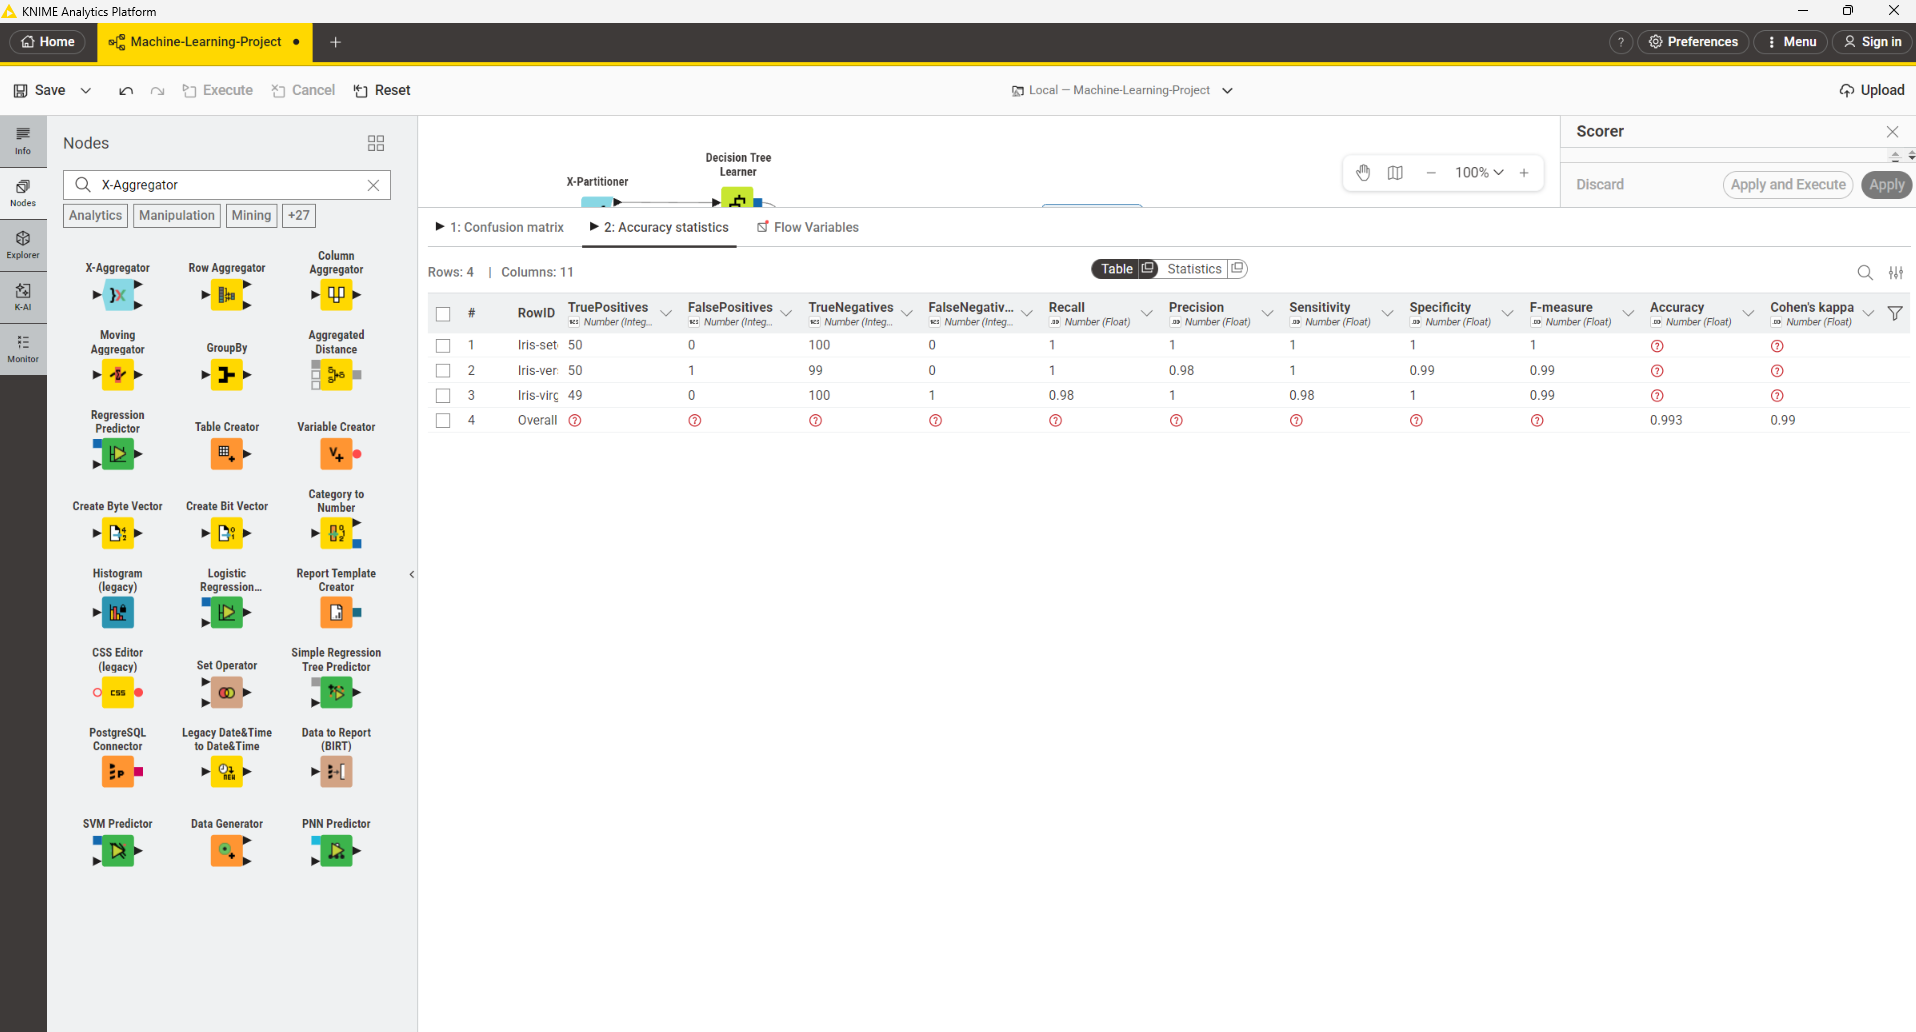
\includegraphics[width=0.95\textwidth]{figures/ml_knime_decision_tree_accuracy.png}
    \caption{Auswertung des Decision-Tree-Modells mit dem KNIME Scorer. Die Gesamtgenauigkeit beträgt 99{,}3\%.}
    \label{fig:knime-decision-tree-accuracy}
\end{figure}

Das Decision-Tree-Modell erreichte eine Gesamtgenauigkeit von \texttt{0{,}993}, was einer Accuracy von \texttt{99{,}3\%} entspricht. Damit wurden nahezu alle Instanzen des Iris-Datensatzes korrekt klassifiziert. Besonders auffällig ist, dass die Klasse \texttt{Iris-setosa} vollständig korrekt erkannt wurde. Dies lässt sich dadurch erklären, dass diese Klasse anhand der Blütenmerkmale deutlich von den anderen beiden Klassen getrennt ist.

Die wenigen Abweichungen treten typischerweise zwischen \texttt{Iris-versicolor} und \texttt{Iris-virginica} auf. Diese Beobachtung ist fachlich plausibel, da sich diese beiden Iris-Arten in ihren Merkmalsausprägungen stärker überlappen als \texttt{Iris-setosa}. Die hohe Modellleistung zeigt, dass ein Entscheidungsbaum für diesen Datensatz gut geeignet ist, da die Klassen anhand weniger Merkmale relativ klar voneinander getrennt werden können.

\subsubsection*{Reflexion}

Die hohe Accuracy zeigt, dass der Iris-Datensatz für ein erstes Klassifikationsexperiment sehr gut geeignet ist. Gleichzeitig darf das Ergebnis nicht überinterpretiert werden, da der Datensatz klein, sauber und stark strukturiert ist. In realen Anwendungsszenarien treten häufig fehlende Werte, unausgewogene Klassen, Rauschen oder komplexere Merkmalsbeziehungen auf. Deshalb wäre ein einzelnes hohes Accuracy-Ergebnis allein nicht ausreichend, um ein Modell als zuverlässig zu bewerten.

Besonders wichtig war in diesem Experiment die Verwendung der Kreuzvalidierung. Im Vergleich zu einer einfachen einmaligen Trainings-Test-Aufteilung liefert die 10-fache Kreuzvalidierung eine stabilere Einschätzung der Modellleistung, da jede Instanz einmal als Testinstanz verwendet wird. Dadurch wird das Risiko reduziert, dass das Ergebnis zufällig durch eine besonders günstige oder ungünstige Datenaufteilung entsteht.

Für mein Verständnis war außerdem wichtig zu sehen, dass ein Machine-Learning-Workflow nicht nur aus dem Training eines Modells besteht. Vor dem eigentlichen Lernen müssen die Daten korrekt importiert, die Zielvariable ausgewählt, die Daten aufgeteilt, Vorhersagen erzeugt und die Ergebnisse kritisch interpretiert werden. Der praktische KNIME-Workflow macht diese Schritte visuell nachvollziehbar.

\subsection{Deep Learning: Lernen mit neuronalen Netzen}


\subsection{Erklaerbare KI: Warum entscheidet ein Modell so?}



\subsection{Vergleich der vier Themen}



\begin{thebibliography}{99}

\bibitem{witten_data_mining}
Witten, I. H. / Frank, E. / Hall, M. A. / Pal, C. J.:
\textit{Data Mining: Practical Machine Learning Tools and Techniques}.
Morgan Kaufmann, 2016.

\bibitem{fayyad_kdd}
Fayyad, U. / Piatetsky-Shapiro, G. / Smyth, P.:
From Data Mining to Knowledge Discovery in Databases.
\textit{AI Magazine}, 17(3), 1996.

\bibitem{han_data_mining}
Han, J. / Kamber, M. / Pei, J.:
\textit{Data Mining: Concepts and Techniques}.
Morgan Kaufmann, 2012.

\bibitem{ibm_data_mining}
IBM:
Was ist Data-Mining?
Online-Artikel.
Verfügbar unter:
\url{https://www.ibm.com/de-de/think/topics/data-mining}
(zuletzt abgerufen am 30.05.2026).

\bibitem{haufe_data_mining}
Haufe Akademie:
Data Mining verstehen: Muster erkennen und Chancen nutzen.
Online-Artikel.
Verfügbar unter:
\url{https://www.haufe-akademie.de/skill-it/blog/data-mining}
(zuletzt abgerufen am 30.05.2026).

\bibitem{inform_data_mining}
INFORM:
Unlocking Data Mining: Insights for Business Success.
Online-Artikel.
Verfügbar unter:
\url{https://www.inform-software.com/en/blog/artificial-intelligence/data-mining-definition-how-it-works-and-examples}
(zuletzt abgerufen am 30.05.2026).

\bibitem{fisher_iris}
Fisher, R. A.:
The Use of Multiple Measurements in Taxonomic Problems.
\textit{Annals of Eugenics}, 7(2), 1936, S. 179--188.

\bibitem{sklearn_iris}
scikit-learn developers:
The Iris Dataset.
Verfügbar unter:
\url{https://scikit-learn.org/stable/auto_examples/datasets/plot_iris_dataset.html}
(zuletzt abgerufen am 30.05.2026).

\bibitem{jier_data_mining_bi}
Journal of Informatics Education and Research:
Data Mining in Business Intelligence \& Decision Making.
Fachartikel, 2023.

\end{thebibliography}
\end{document}